\begin{enumerate}
	\item Conceito e exemplos de informação binaria: 
	\begin{enumerate}
		\item Uma fogueira avisando a tribo que o inimigo se aproxima, ou que a tribo conseguiu comida.
		\item Torres de vigilancia na Grande Muralha da China.
	\end{enumerate}
	\item Experimentos na protoboard explicados na lousa:
	\begin{enumerate}
		\item Led e botao.
		\item Led e \textbf{!}botao.
		\item Porta AND com 2 botões.
		\item Porta OR com 2 botões.
		\item Outras variacões e experimentos que o professor achar conveniente.
	\end{enumerate}
\end{enumerate}

\vfill

\begin{center}
	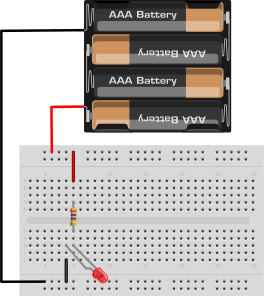
\includegraphics[height=.9\textheight]{./IMG/LED_bb.png}
\end{center}

\vfill
\begin{itemize}
	\item N.O. Push button: 0==0
	\item N.C. Push button: 0=!1
\end{itemize}
\begin{center}
	\includegraphics[height=.8\textheight]{./IMG/LED_bb-button.png}
\end{center}

\vfill\columnbreak

{\Large A \textbf{\&\&} B}
\begin{center}
	\includegraphics[height=.8\textheight]{./IMG/LED_bb-and.png}
\end{center}

\vfill\columnbreak

{\Large A \textbf{\textbar\textbar} B}
\begin{center}
	\includegraphics[height=.8\textheight]{./IMG/LED_bb-or.png}
\end{center}

\vfill\columnbreak